%% ============================================================
\chapter{Experiments and Results}
\label{ch:results}
%% Target length: ~25 pages (main results chapter, formatted as manuscript)
%% Can be structured as a self-contained paper following Nature Methods style
%% (as Jelle did in Ch. 6), or as conventional subsections.
%% Recommend conventional subsections for the thesis; paper can be appendix.
% Our experiments are focused on decreasing the latency to achieve real time super resolution reconstructions
% while maintaining the accuracy high.
% % Sections~\ref{ssec:transformer_sizes} and \ref{ssec:N-frame Fusion}

% First, we compare different sizes of TRNet fusion module in Section~\ref{ssec:transformer_sizes},
% the effect of increasing the number of input frames into pretrained TRNet in 
% Section~\ref{ssec:N-frame Fusion}


% \begin{itemize}
%   \item Decoder ablation: PixelShuffle vs. ConvTranspose2d (Section~\ref{sec:decoder_ablation})
%   \item Loss function comparison: Fourier, L1\_Fourier (Section~\ref{sec:loss_compare})
  
%   \item Training set size effect analysis (Section~\ref{sec:dataset_size})
%   \item TRNet\_improved: FlashAttention and CrossAttentionAggregator (Section~\ref{sec:improved})
%   \item Inference speed and latency benchmarking (Section~\ref{sec:latency})
%   \item Transformer size comparison (Section~\ref{sec:transofmer_size_compare})
% \end{itemize}

% And quantitative analysis to evaluate performance against the foundational models from RESURF \cite{resurf2024}.
% \begin{itemize}
%   \item Architecture comparison: TRNet vs. SOFI-MISRGRU (Section~\ref{sec:arch_compare})
%   \item Streaming MISRGRU evaluation and deployment feasibility (Section~\ref{sec:streaming})
% \end{itemize}




\section{How good is TRNet?}
\label{sec:arch_compare}

\subsection{Experimental Setup}
\label{ssec:experimental_setup}

\subsubsection{Model Training Details}
All TR-MISR experiments use the improved TRNet architecture with a PixelShuffle decoder
and a lightweight fusion module (1 attention head, depth 1), trained on 8 input frames.
Models are optimised with Adam using a learning rate of $10^{-3}$ for the encoder/decoder
and $5 \times 10^{-4}$ for the transformer, reduced on validation-loss plateau.
The combined L1+Fourier loss is used throughout; 2000 simulated samples are used with a
90/10 train/validation split. The choice of loss function and decoder were
validated by ablation; see Appendix~\ref{app:trnet_modifications}.

The test set comprises 12 SNR conditions spanning three blinking speeds
(fast, medium, slow) and four photon levels (100\%, 80\%, 60\%, 40\% of nominal),
with 40 samples per condition (480 test samples total).

\subsection{Evaluation Metrics}
\label{ssec:metrics}

Standard pixel-level metrics such as MSE, PSNR, and SSIM are poorly suited for evaluating
super-resolution SOFI reconstructions. As noted by~\cite{jelle2024}, SOFI images are
dominated by near-zero background pixels, so averaging errors over all pixels yields an
overly optimistic assessment even when fine structural detail is poorly reproduced.
We instead adopt two metrics used by~\cite{resurf2024}, enabling direct comparability.

\textbf{Resolution-scaled Pearson correlation (RSP).}
RSP measures the Pearson correlation between a predicted SR image and a reference image,
after the SR image has been rescaled in both resolution and intensity to match the reference.
The rescaling corrects for differences in sharpness between prediction and reference, so
RSP reflects structural agreement rather than penalising the model for being sharper than
the reference. RSP lies in $[-1,\,1]$; values closer to~1 indicate better structural
fidelity. When the ground-truth SOFI image is available (simulated test set), it is used
as the reference.

% \textbf{SQUIRREL.}
% The resolution and intensity rescaling required to compute RSP is performed by the
% SQUIRREL algorithm~\cite{culley2018squirrel}. SQUIRREL iteratively estimates a
% point-spread function (PSF) by convolving the SR image and comparing to the reference
% until the convolved SR best matches the reference. In addition to the RSP score, SQUIRREL
% produces pixel-wise RSE (resolution-scaled error) maps that visualise local deviations
% and are useful for identifying spatial regions where the model introduces artefacts or
% misses structure.

\textbf{Decorrelation analysis\textcite{descloux2019decorrelation},} is commonly used in 
SR microscopy to estimate spatial resolution directly from each output image without 
requiring a ground truth.
The normalised Fourier transform is cross-correlated with the input image through a binary
circular mask of shrinking radius $r \in [0,1]$.
A peak in the resulting curve $d(r)$ identifies the highest spatial frequency carrying
coherent signal. Repeating over a series of high-pass filters and taking the maximum peak
position $k_c$ gives the cut-off frequency, from which resolution is computed as:
\begin{equation}
  \text{Resolution} = \frac{2 \times \text{pixel size}}{k_c}.
  \label{eq:decorrelation_resolution}
\end{equation}
This parameter-free estimate yields the achieved spatial resolution in nanometres,
complementing the structural-fidelity measure provided by RSP.

\begin{figure}[h]
  \centering
  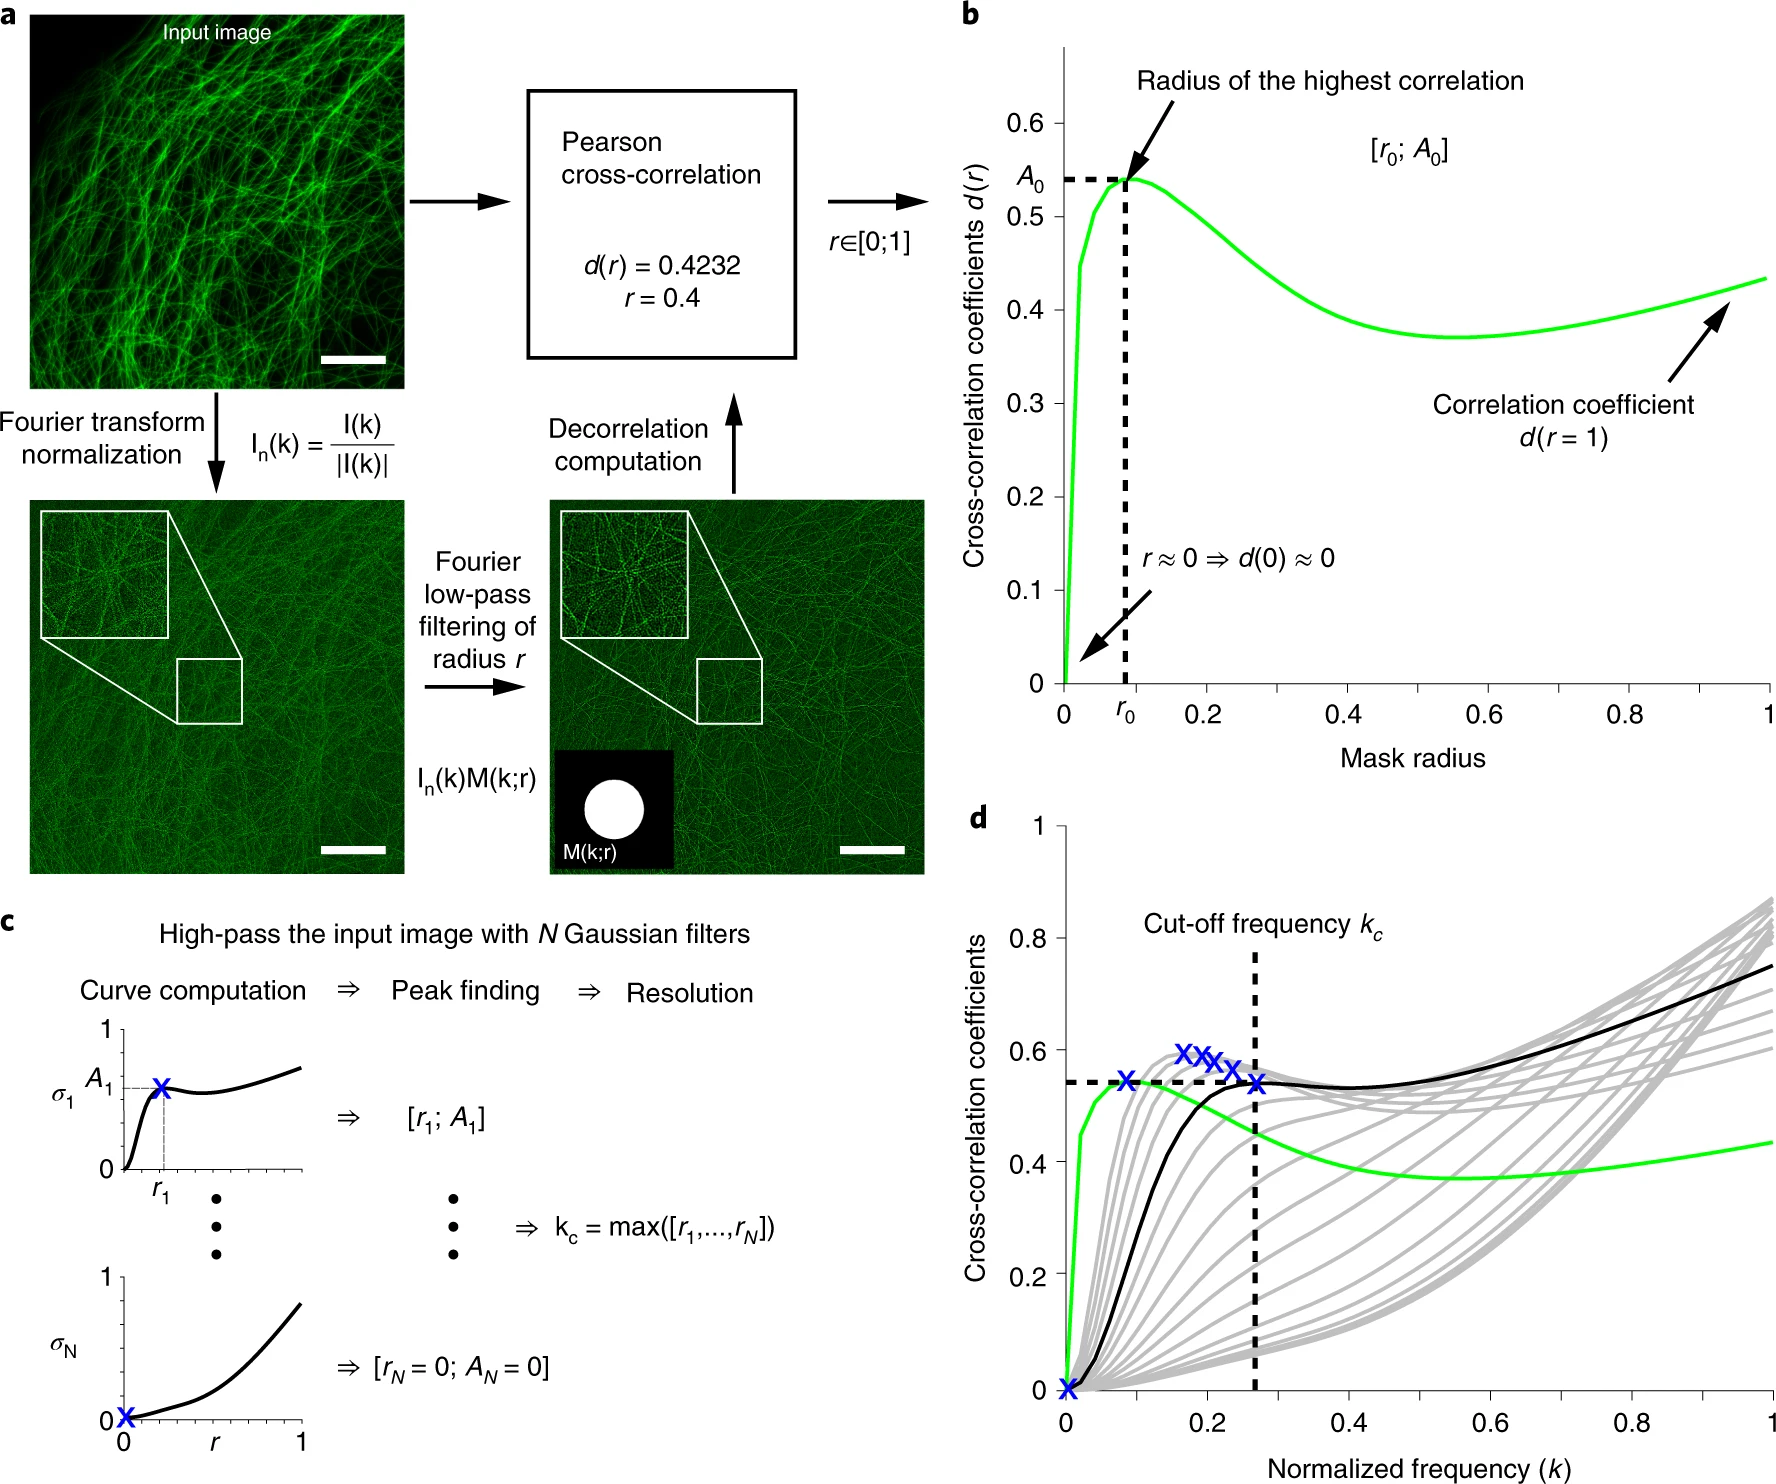
\includegraphics[width=0.75\linewidth]{figures/decorr_algorithm.png}
  \caption{}
  \label{fig:decorr_algorithm}
\end{figure}

RSP is the primary metric reported in all experiments; decorrelation analysis is reported
only for the best models of each class. 


\subsection{Multi-frame Fusion}
\label{ssec:multi-frame Fusion}

Because TR-MISR's cross-attention aggregator uses a softmax over all $T$ input tokens, it
is not architecturally constrained to a fixed frame count.
A model trained on 8 frames can therefore attend to longer sequences at test time without
retraining or fine-tuning. Sequential GRU fusion does not share this capability as shown in the experiment.

To verify this, we evaluate the same 8-frame pretrained 1h1d model at
$N \in \{8, 20, 30\}$ input frames and compare against the MISRGRU foundational models
from RESURF~\cite{resurf2024}.
Figure~\ref{fig:boxplot_rsp_model_comparison} shows RSP aggregated over all 480 test
samples, with classical SOFI (100-frame) shown in grey as an upper reference.

\begin{figure}[h]
  \centering
  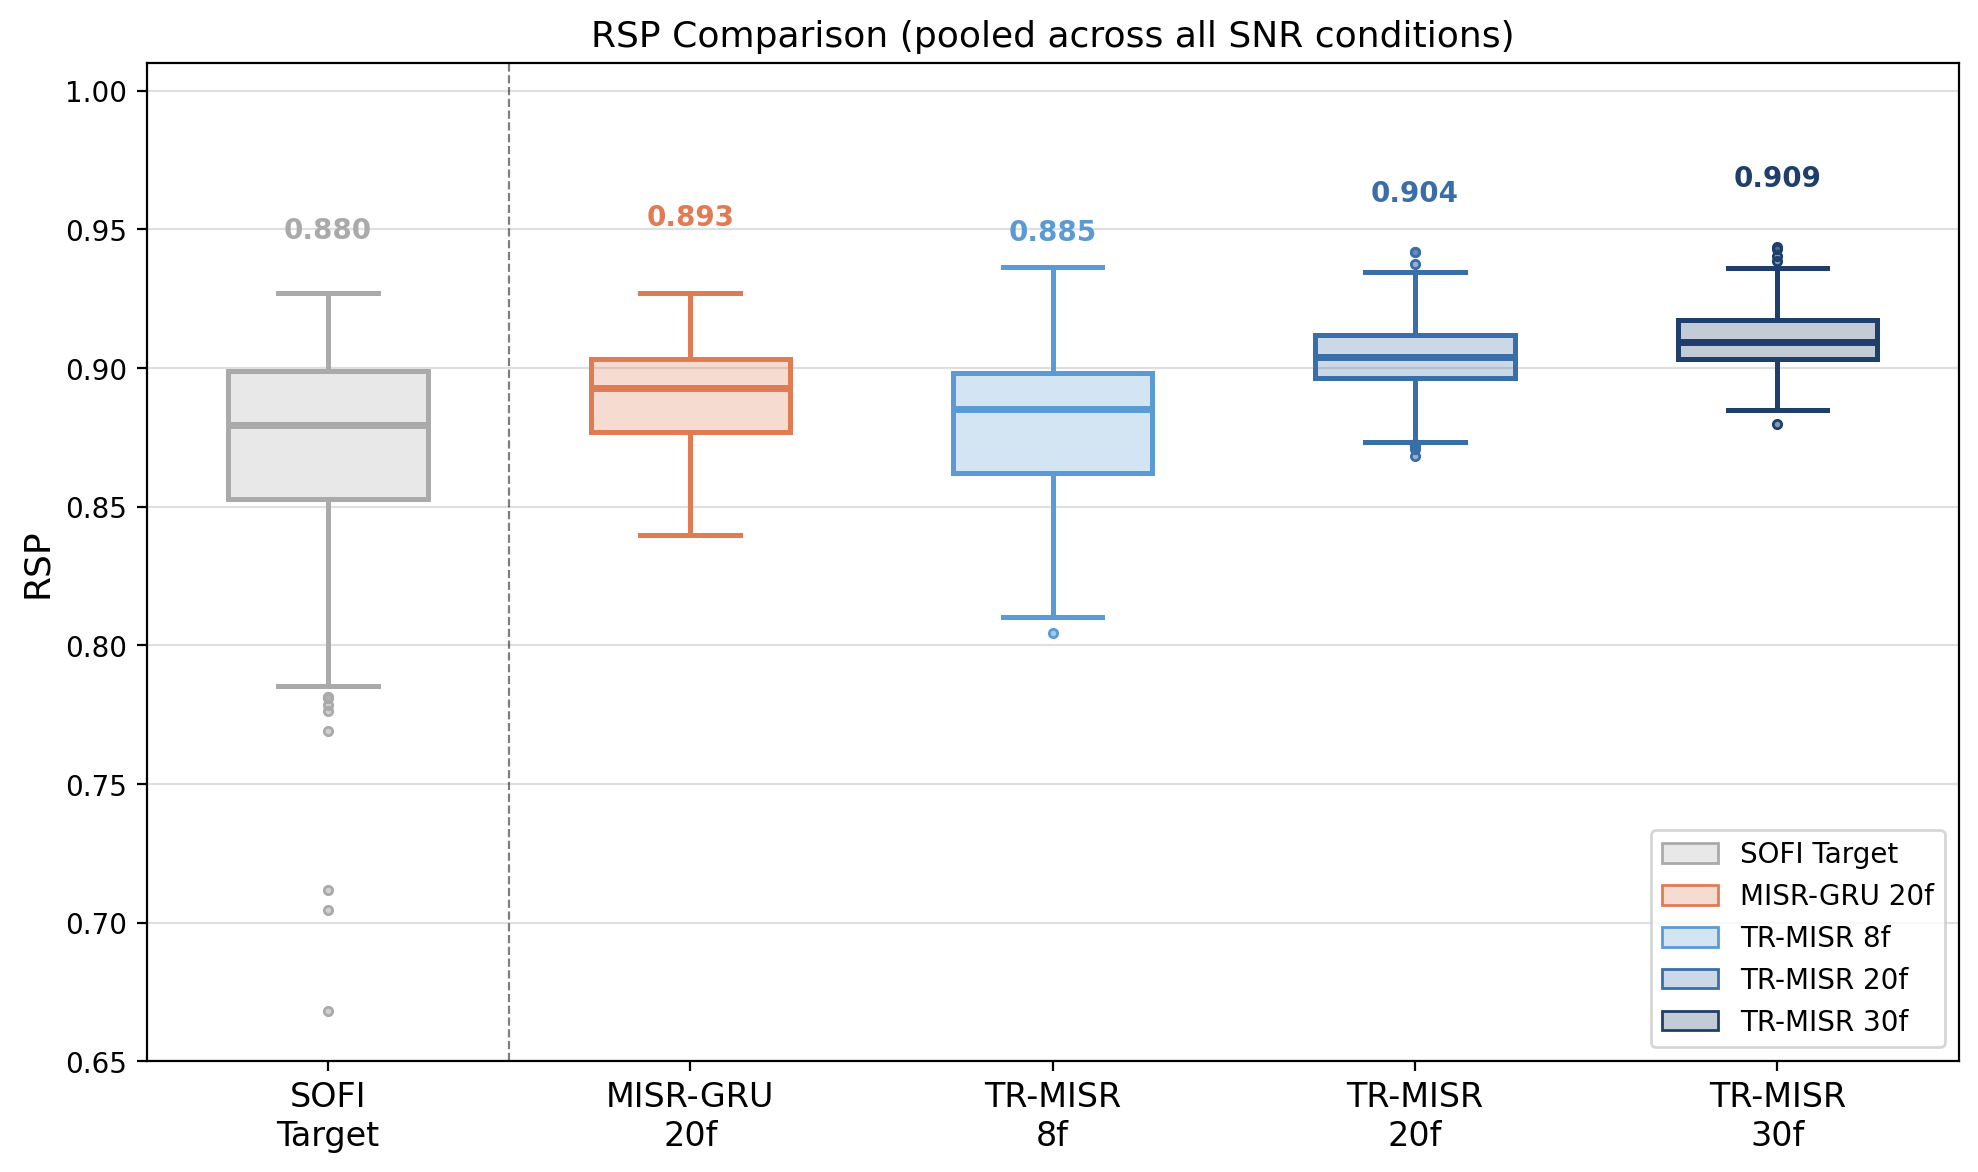
\includegraphics[width=0.8\linewidth]{figures/boxplot_rsp_comparison_models_sofi.png}
  \caption{RSP distribution for TR-MISR 1h1d at 8, 20, and 30 input frames versus
  the best MISRGRU 20-frame foundational model from RESURF~\cite{resurf2024}.
  Classical SOFI (100-frame) is shown in grey as an upper reference.}
  \label{fig:boxplot_rsp_model_comparison}
\end{figure}

Providing more frames consistently improves TR-MISR: the 20-frame and 30-frame variants
both exceed the MISRGRU 20-frame baseline in aggregate RSP shown in 
Figure~\ref{fig:boxplot_rsp_model_comparison}.

This confirms that the attention mechanism generalises to sequences longer than
those seen during training.

Figure~\ref{fig:n_frame_fusion} breaks results down per SNR condition.
MISRGRU is more consistent across conditions: its inter-quartile range is tighter at
high-SNR settings (fast blinking, high photon counts).
TR-MISR, however, degrades less at low SNR: under slow-blinking and low-photon
conditions (09--12\_slow), TR-MISR's median RSP stays closer to the 8-frame MISRGRU
baseline, whereas MISRGRU 8f falls more sharply.

\begin{figure}[h]
  \centering
  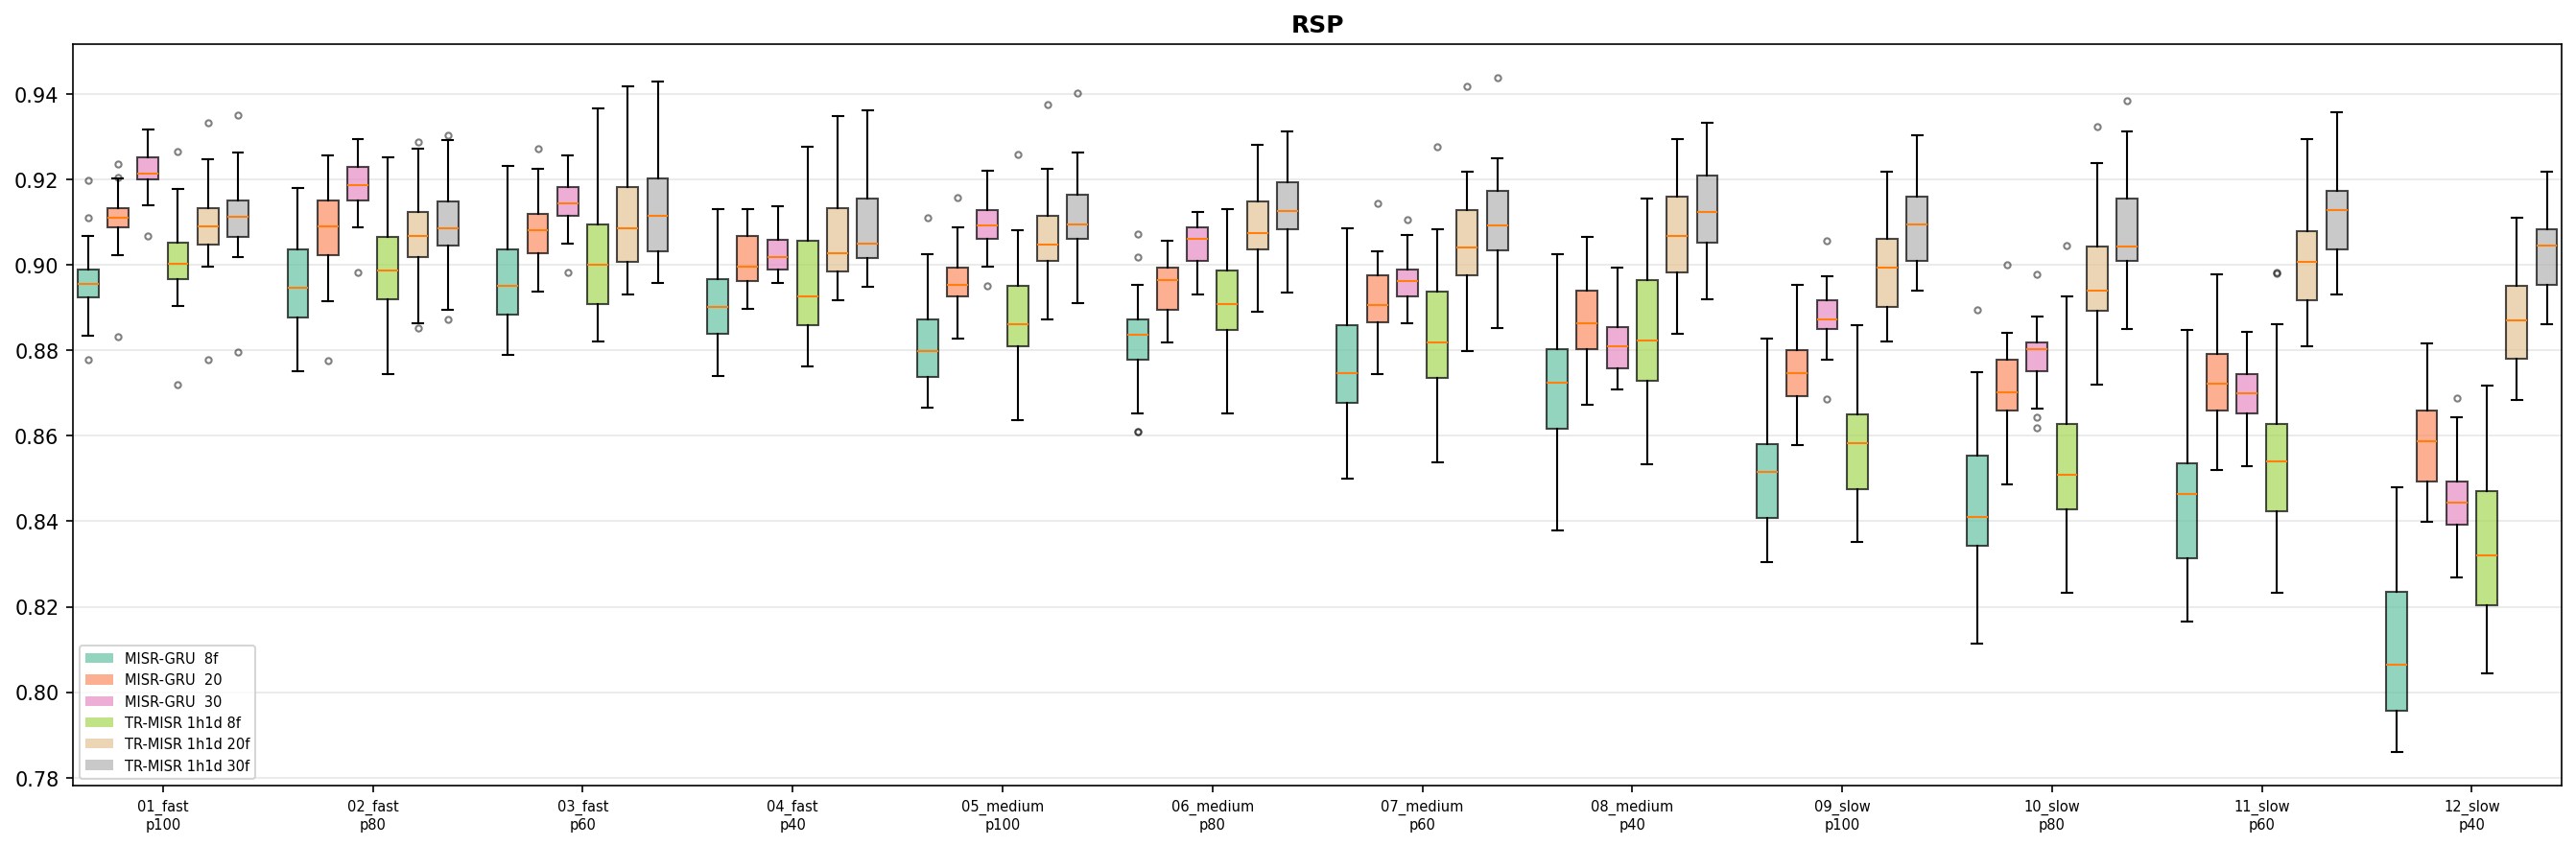
\includegraphics[width=0.8\linewidth]{figures/n_frame_comparison.png}
  \caption{RSP per SNR condition (blinking speed $\times$ photon level) for TR-MISR 1h1d
  at 8, 20, and 30 frames and MISRGRU baselines. Conditions are ordered fast\,$\to$\,slow
  blinking and 100\%\,$\to$\,40\% photon level within each speed group.}
  \label{fig:n_frame_fusion}
\end{figure}

Surprisingly, the MISRGRU 20-frame model performs worse on
several slow-blinking conditions when the input is extended to 30 frames.
We attribute this to the unnormalised summation in the fusion module's GAP layer, which
causes the decoder input magnitude to grow with $T$ beyond the range seen during training.
Section~\ref{ssec:kbuf_misrgru} analyses this effect quantitatively.


\subsection{Effect of Training Frame Count: 8f vs 20f TRNet}
\label{ssec:trnet_8f_vs_20f}

To understand whether training on more frames improves TRNet, we trained an additional
model on 20-frame sequences and compared it against the 8-frame trained model across
$N \in \{20, 30\}$ input frames at test time.
Figure~\ref{fig:boxplot_rsp_20fvs8f} shows the RSP distributions for both models.

\begin{figure}[h]
  \centering
  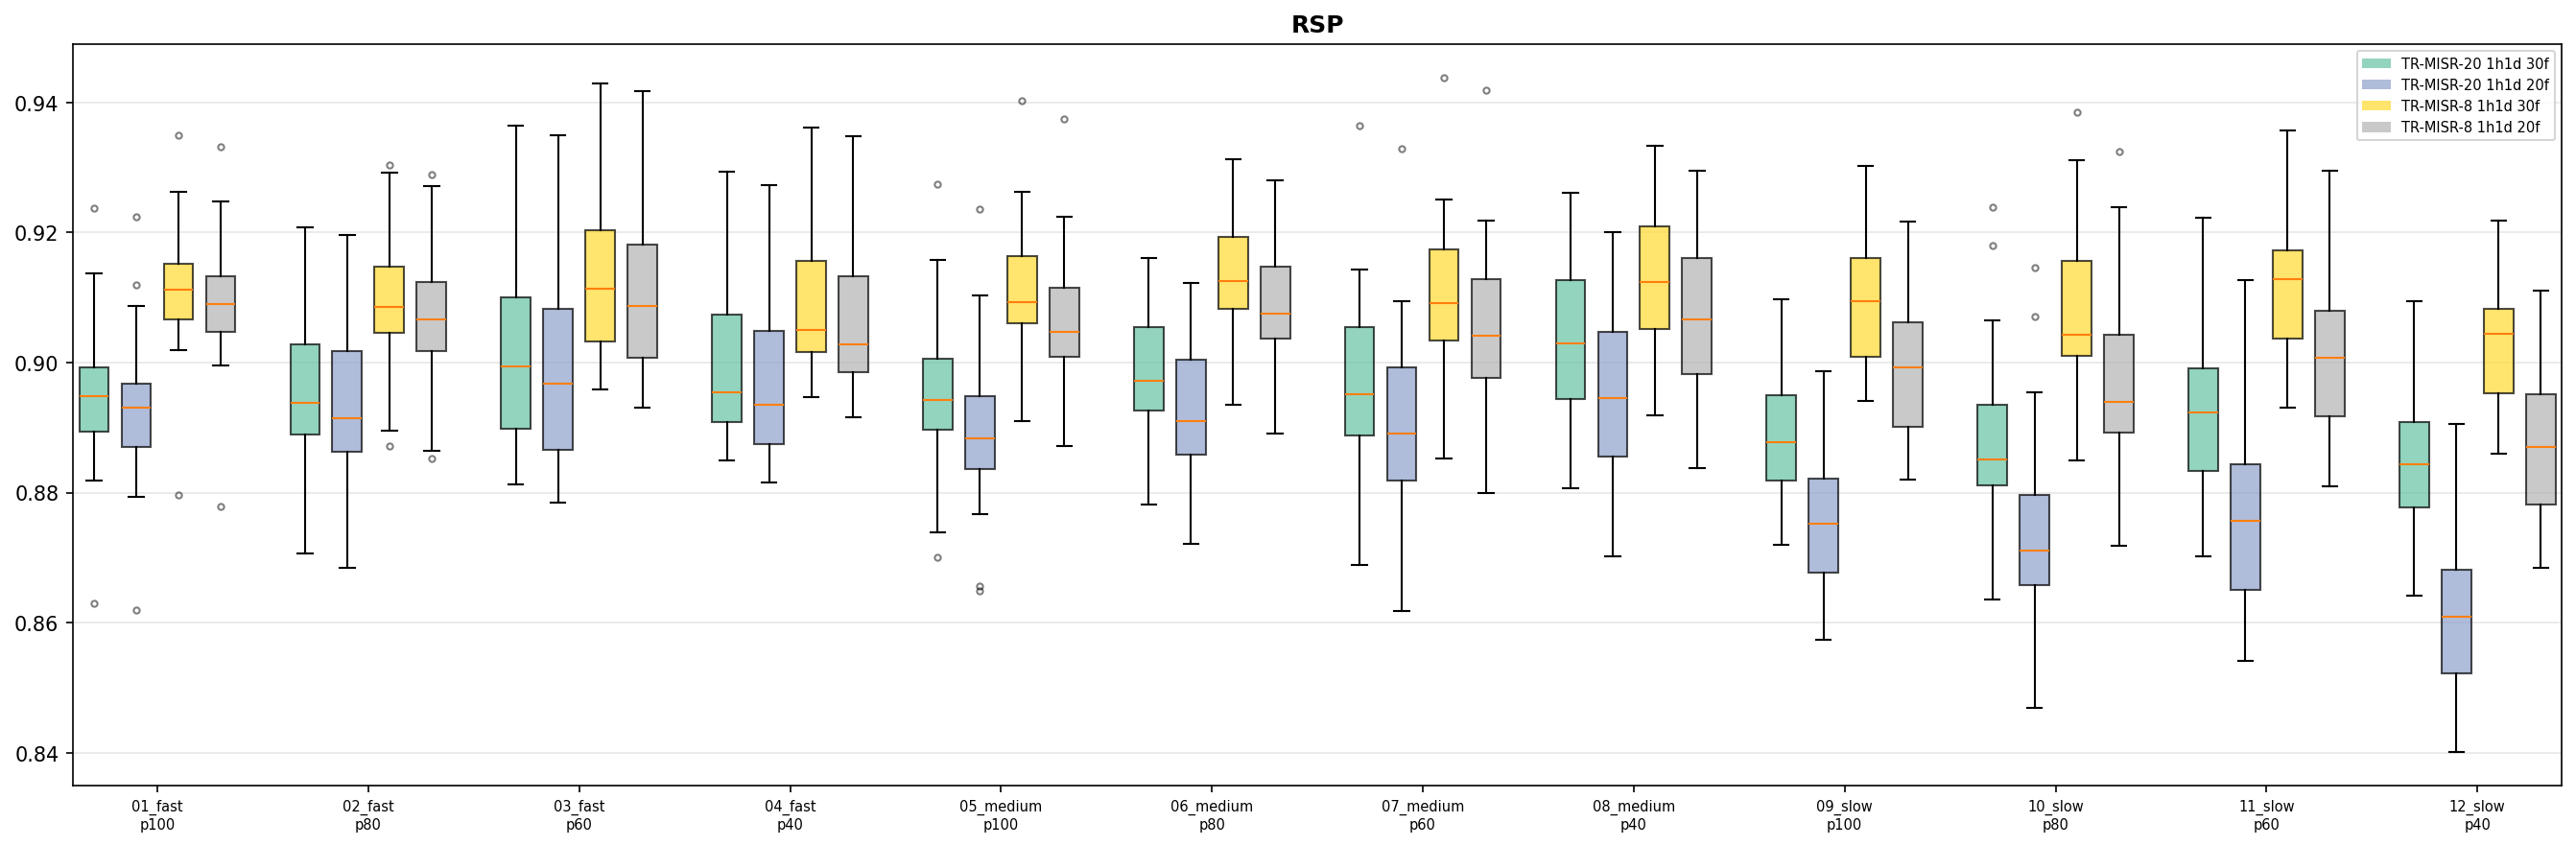
\includegraphics[width=0.8\linewidth]{figures/boxplot_rsp_20fvs8f_trnet.png}
  \caption{RSP distribution for TRNet trained on 8 frames versus TRNet trained on 20 frames,
  evaluated at 20, and 30 input frames at test time. The 8f-trained model outperforms
  the 20f-trained model when both are given 20 or 30 frames on all SNR conditions.}
  \label{fig:boxplot_rsp_20fvs8f}
\end{figure}

Counterintuitively, the 8-frame trained model outperforms the 20-frame trained model when
both are evaluated on 20 and 30 input frames.
We belive that 8 frames is already sufficient to capture the temporal correlations produced by
fluorophore blinking: at the simulated acquisition rates and blinking speeds, most
fluorophores will have switched state at least once within 8 frames, so the cross-attention
module receives a diverse sample of blink events and can learn a sharp aggregation.
Training on 20 frames does not provide fundamentally new blinking statistics; it
predominantly adds redundant observations of the same fluorophore states.

Second, with 20 training frames the attention module may become \emph{over-saturated} at
individual spatial locations: a fluorophore that is on for many consecutive frames
produces a cluster of similar tokens that dominates the cross-attention, potentially
suppressing weaker but informative blink events elsewhere.
The 8-frame model, having learned to aggregate under a tighter budget, develops attention
weights that are more robust to token redundancy, which is why it generalises better when
the sequence is extended at test time.

This finding reinforces the conclusion from Section~\ref{ssec:multi-frame Fusion}: the
attention mechanism benefits from being given more frames at inference, but the model
should be \emph{trained} on a short sequence to encourage efficient use of each frame.

\subsection{Decorrelating 8f TRNet model}
To verify that frame-count generalisation does not degrade output resolution,
we apply decorrelation analysis~\cite{descloux2019decorrelation} to the SR outputs of each MISRGRU
variant across all four blinking regimes: fast-high SNR (FH), fast-low SNR (FL),
slow-high SNR (SH), and slow-low SNR (SL).
Decorrelation analysis estimates the resolution directly from a single image
by measuring how quickly spatial autocorrelation decays with increasing frequency,
yielding a resolution figure in nanometres that is independent of the ground-truth target.

Figure~\ref{fig:imdecor_8f} shows box plots of the estimated resolution for
model trained on 8 frames but evaluated at 8, 20 and 30 input frames, 
each evaluated on 12 SNR test conditions grouped into the four regimes above.
All three variations are able to resolve structure well below the optical diffraction limit
(${\approx}250$\,nm for visible light), confirming genuine super-resolution across
all blinking configurations.

Within each model, the fast-blinking conditions yield sharper outputs than the
slow-blinking ones.
The FL condition consistently achieves the lowest (best) median resolution
estimates across all models.

Comparing the three variants, the 8-frame model produces the tightest distributions
under the SH and SL regimes, while the 20-frame and 30-frame variants
exhibit marginally wider spread.

\begin{figure}[h]
  \centering
  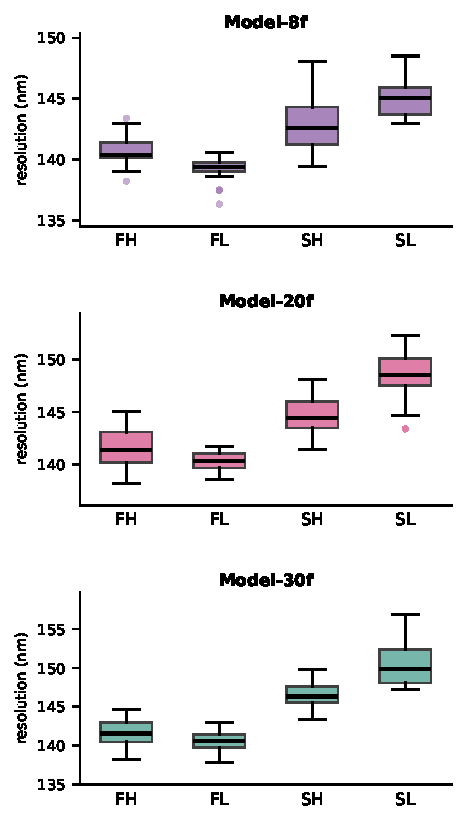
\includegraphics[width=0.4\linewidth]{figures/imdecor_8f_trained_8_20_30.pdf}
  \caption{Decorrelation analysis of MISRGRU outputs for models trained on 8, 20,
           and 30 frames across four blinking/SNR conditions.
           Lower resolution values indicate sharper, higher-fidelity super-resolved images.
           All models resolve below the diffraction limit (${\approx}250$\,nm).}
  \label{fig:imdecor_8f}
\end{figure}

\subsection{Latency vs Transformer Size Trade-offs}
\label{ssec:latency_transformer_sizes}

To figure out the best accuracy speed tradeoff of the TR-MISR model we trained four 
different models where we varied the sizes of heads and depths used in transformer fusion module.
Figure~\ref{fig:transformer_sizes} depicts the evaluation of different using RSP metric.
Increasing the number of parameters does not improve the metric dramatically, suggesting the
fusion module reaches capacity quickly and that a single attention head with one 
transformer layer (1h1d) is sufficient to aggregate cross-frame information    
making it the preferred configuration given its substantially lower inference latency 
(Table~\ref{tab:inference_latency}). The encoder/decoder are the limiting factor.

\begin{figure}[h]
  \centering
  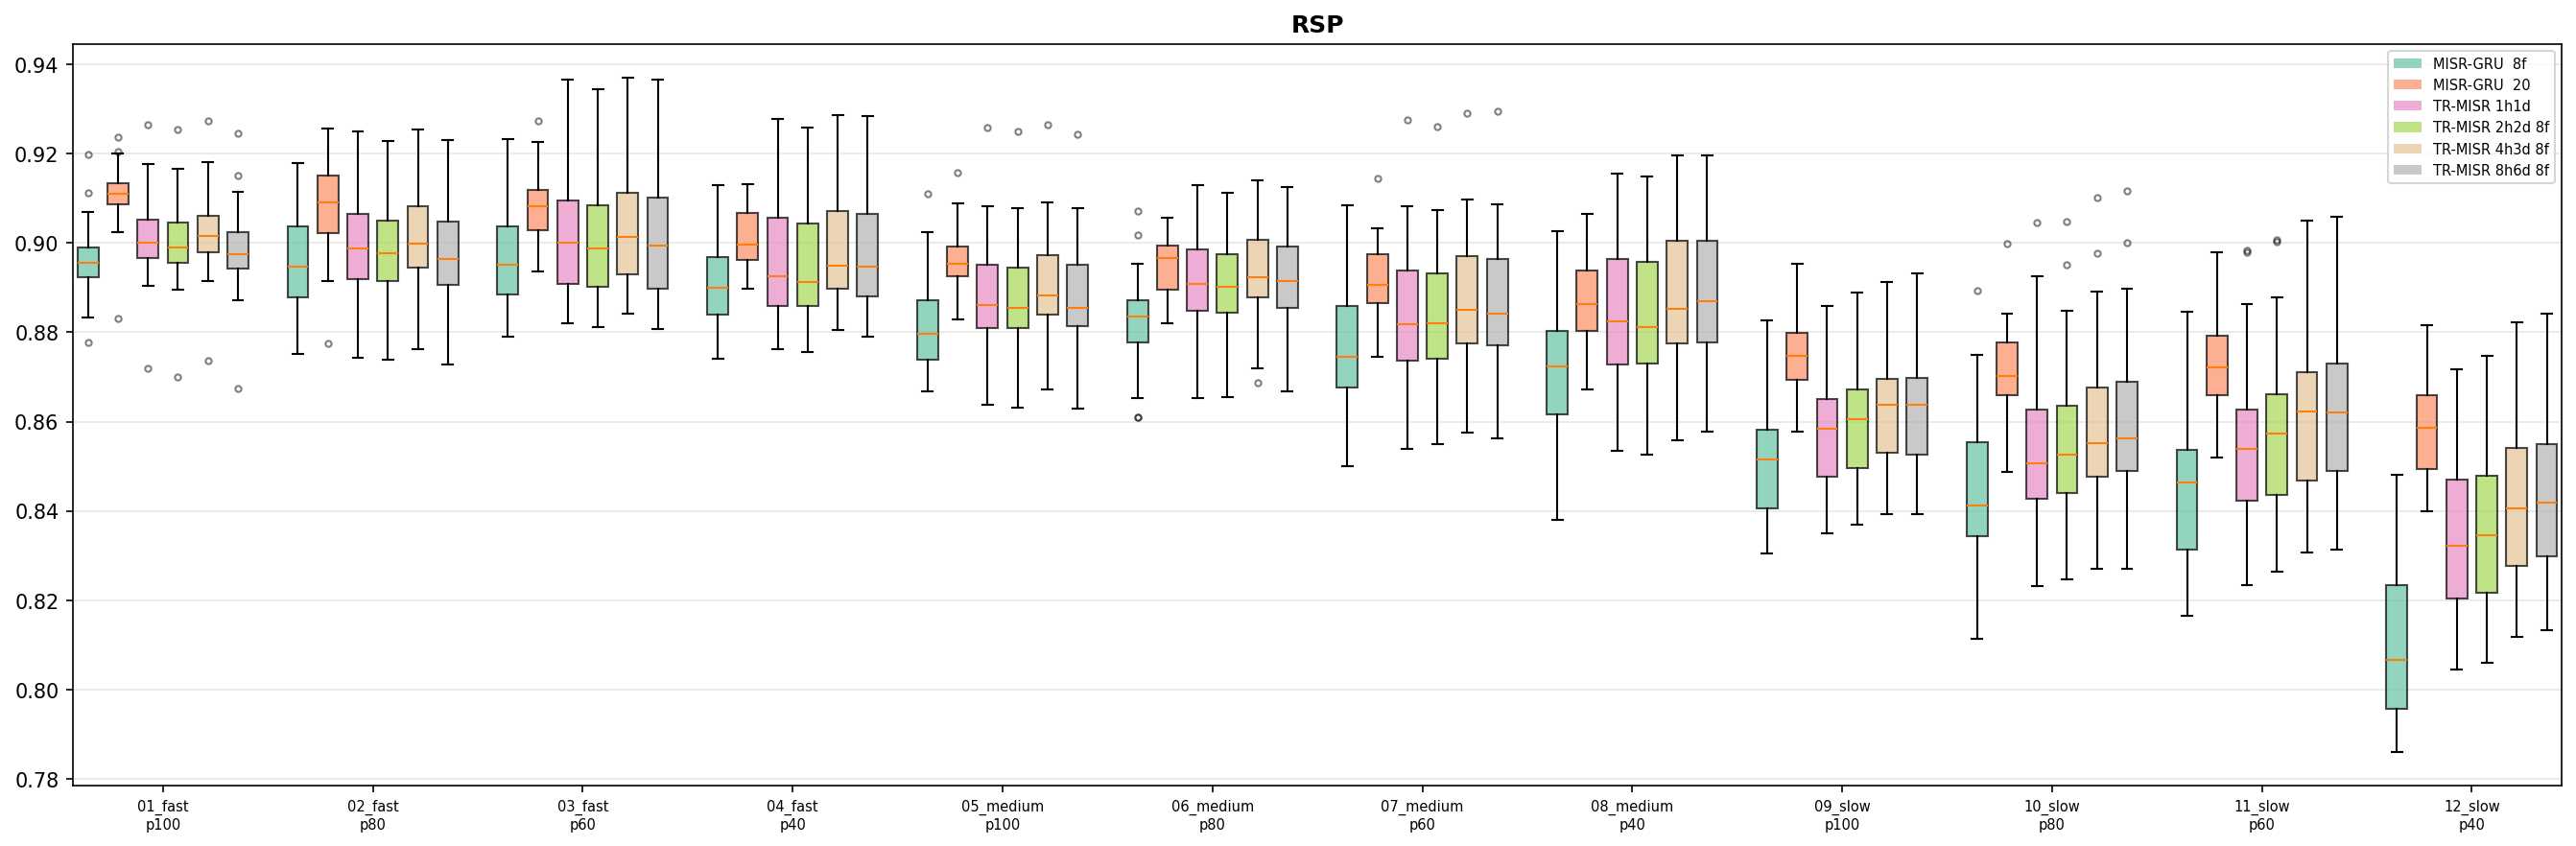
\includegraphics[width=0.8\linewidth]{figures/transformer_size_ablation_rsp.png}
  \caption{Resolution-scaled Pearson correlation for four Transformer configurations with 
  varying depth and attention heads across SNR conditions. Baseline MISRGRUs (pre-trained 8 and 20 frames) 
  are shown as for reference.}
  \label{fig:transformer_sizes}
\end{figure}

To assess the computational cost and speed of TRNet, experiments with increasing Transformer 
depth and attention heads, were done.
We benchmarked all four TR-MISR size variants and the MISRGRU baseline on an NVIDIA RTX A5000 
(24\,GB) using PyTorch and TensorRT execution. \todo{add tesnort graph}
Each model was evaluated at three frame counts ($N \in \{8, 20, 30\}$) where the frame size 
was 512x512 pixels. 8 frames matches the MISRGRU baseline, 20 frames is the best performing 
foundational model in prior work, and 30 frames tests scalability.

\begin{table}[h]
  \centering
  \caption{Model parameter counts and PyTorch inference latency on 512×512 images 
  (mean over 100 runs). Measurements on NVIDIA RTX A5000 with batch size 1. 
  Fastest inference time per frame count is highlighted in bold.}
  \label{tab:inference_latency}
  \begin{tabular}{lrccc}
    \hline
    \textbf{Model} & \textbf{Params} & \textbf{N=8 (ms)} & \textbf{N=20 (ms)} & \textbf{N=30 (ms)} \\
    \hline
    TR-MISR 1h1d  &  \textbf{48,692} & 87.97 & 262.55 & 608.56 \\
    TR-MISR 2h2d  &  57,388 & 188.14 & 487.61 & 1200.65 \\
    TR-MISR 4h3d  &  66,084 & 209.10 & 858.60 & 3935.62 \\
    TR-MISR 8h6d  & 145,932 & — & — & — \\
    MISRGRU       &  95,073 & \textbf{67.64} & \textbf{170.29} & \textbf{255.92} \\
    \hline
  \end{tabular}
\end{table}

Latency scales super-linearly with transformer depth and head count: going from 1h1d          
to 4h3d triples the parameter count but increases N=8 latency by 2.4× (87.97\,ms to           
209.10\,ms), while 8h6d could not be evaluated within the available memory budget.            
MISRGRU remains the fastest model at every frame count largerly because of it purely convolutional      
fusion mechanism, which avoids the quadratic attention computation over the spatial sequence.      
                                                                                              
Looking at both, the RSP scores (Figure~\ref{fig:transformer_sizes}) and latency               
measurements (Table~\ref{tab:inference_latency}) lead to the same conclusion: the             
transformer fusion module saturates at minimal capacity. Quality does not improve             
meaningfully beyond 1h1d, yet latency grows steeply with model size. For real-time            
live-cell imaging at 40\,fps (25\,ms budget per frame), TR-MISR 1h1d at N=8 is the            
only TR-MISR variant that remains feasible. All subsequent experiments therefore use          
the 1h1d configuration.

\todo{real data experiments with squirel}
\todo{training set size ablation}

\section{Modifying MISRGRU to for video SR reconstruction}

\subsection{Sliding-window MISRGRU modification for faster inference}
\label{ssec:kbuf_misrgru}

Subsection~\ref{ssec:multi-frame Fusion} claimed that MISRGRU oversaturates the input into the 
decoder and quality of the output degrades with the increasing number of frames. 
In this experiment we took pretrained weights from foundational models and modified the architecture
to reuse the outputs $h_t$ from convolution gru layers. We kept the weights in a queue of size 20.

The figure~\ref{fig:kbuf_degradation} shows this empirically with RSP metric as increasing number
of frames are input into the model. The model is evaluated at 1, 5, 10, 20, 40, 80, and 100 
input frames.

This experiment showed us that MISRGRU architecture with summative GAP layer is not well 
suited for multi-input-multi-output task which prompted us to change the architecture to streaming MISRGRU
which normalizes the input in the decoder to produce consistent results.

\begin{figure}[h]
  \centering
  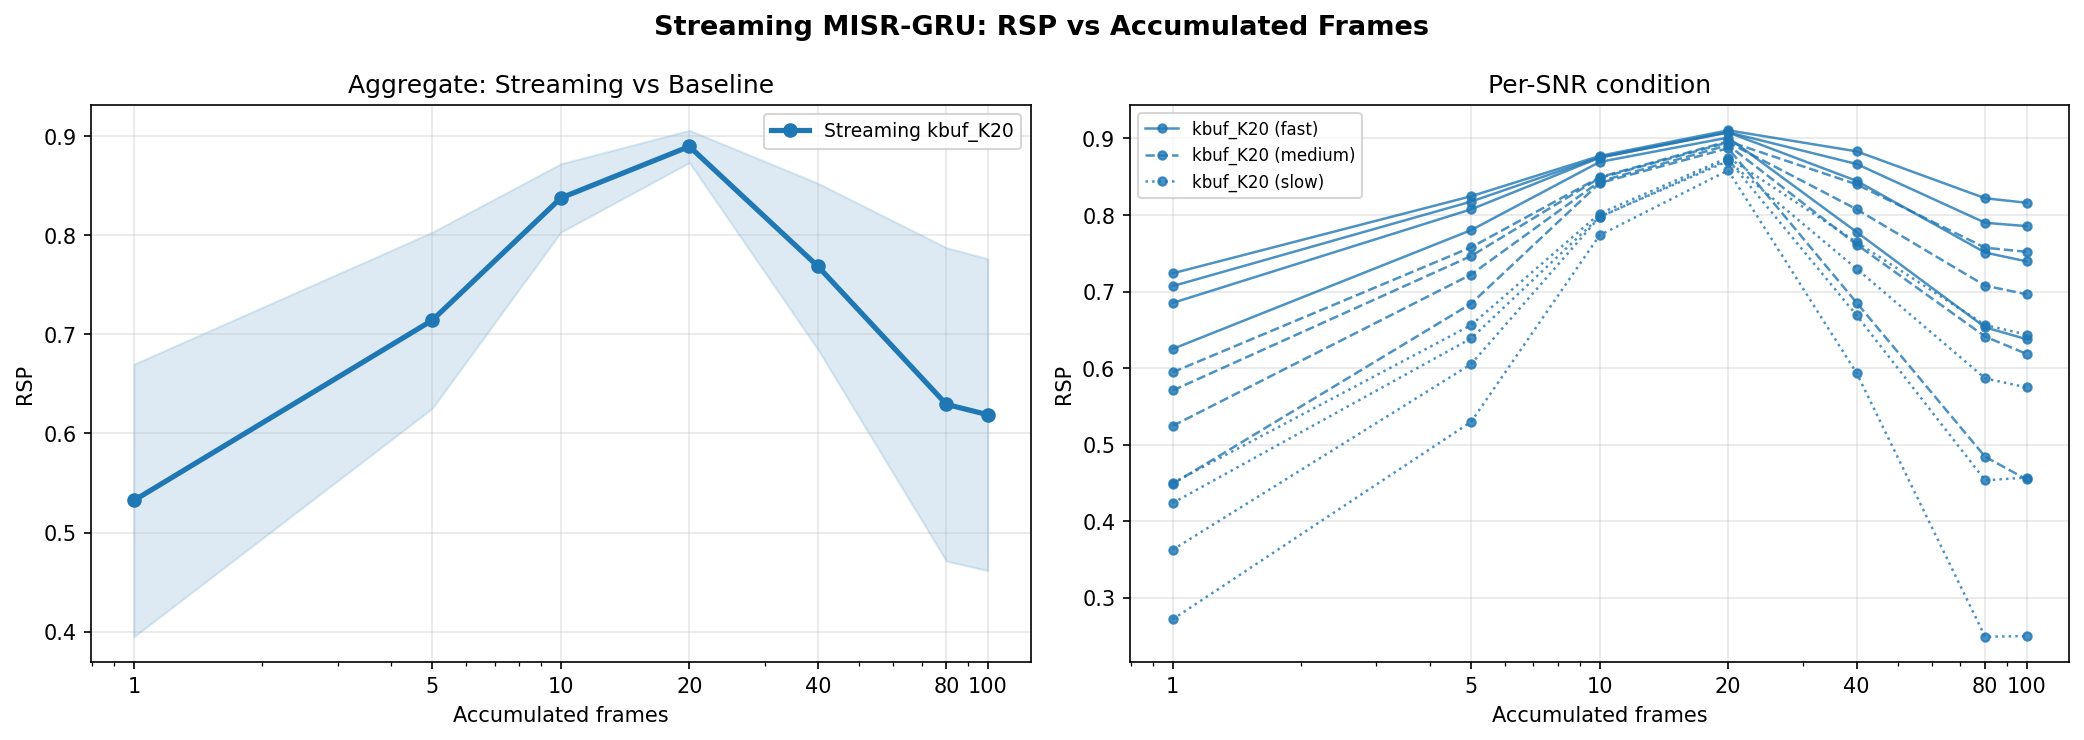
\includegraphics[width=1.0\linewidth]{figures/kbuf_degradation.png}
  \caption{Degrading output quality of K-buffer MISRGRU modification.}
  \label{fig:kbuf_degradation}
\end{figure}


The GRU hidden state $h_t$ is a cumulative summary of all frames up to time $t$,
so the fused representation $\mathbf{f} = \sum_{t=0}^{T-1} h_t$ is an unnormalised
accumulation: the first frame contributes to every $h_t$, giving it $T$-fold weight
relative to the final frame.
Moreover, $h_t$ tends to grow in magnitude, making the sum grow with $T$.
A decoder trained on 20 input frames therefore receives activations of a different
scale when the number of input frames is extended changed at test time.

To verify this claim empirically, we measured the L2-norm of the tensor passed to
each model's decoder ($f$) on 20 real microscopy patches from the testing set,
changing the number of input frames $T \in \{8, 20, 30\}$.
The results are reported in Table~\ref{tab:decoder_input_norm}.
For both MISRGRU variants the decoder-input norm scales beyond the linear
expectation, confirming the saturation hypothesis. 
In contrast, TR-MISR's fusion output remains almost constant across all
three frame counts (ratios of $1.02\times$ and $1.01\times$), because the
cross-attention softmax redistributes weight across frames rather than accumulating
magnitude. Interestingly 8 frame MISRGRU at $T=8$ reaches approximately same L2 norm as the
20 frame MISRGRU at $T=20$ indicating that both models decoder learnt to input similar tensor.

\begin{table}[h]
  \centering
  \caption{Mean L2-norm of the decoder input $f$ on 20 test patches ($256\times256$)
           as the number of input frames $T$ varies.}
  \label{tab:decoder_input_norm}
  \begin{tabular}{lrrrcc}
    \toprule
    \textbf{Model} & \textbf{Train $T$}
      & $\|\mathbf{f}\|_2\ (T{=}8)$
      & $\|\mathbf{f}\|_2\ (T{=}20)$
      & $\|\mathbf{f}\|_2\ (T{=}30)$ \\
    \midrule
    MISRGRU        & 20 & 671  & 2\,741 & 5\,786  \\
    MISRGRU        &  8 & 2\,227 & 8\,194 & 12\,420 \\
    TR-MISR (1h1d) &  8 & 194  & 198    & 200     \\
    \bottomrule
  \end{tabular}
\end{table}


TR-MISR does not suffer from this issue because its cross-attention aggregator normalises
encoded information from all $T$ frames with a softmax.
Adding more frames redistributes attention weight rather than increasing output magnitude,
so the decoder always receives a input at consistent scale regardless of
how many frames are input.
Furthermore, when $T$ exceeds the training length, positional embeddings are linearly
interpolated, allowing the model to generalise to larger input
sets without retraining and train faster and more efficient with less input frames.




\section{Streaming MISRGRU}
\label{sec:streaming}
Streaming models are evaluated by feeding frames one at a time from the test set and measuring 
RSP between the current SR output and the ground truth SOFI image. 
We report RSP metric as a function of the number of accumulated frames at checkpoints 
$\{8, 20, 40, 100\}$, per each of 12 SNR conditions and all test samples. 
Two batch-mode baselines are included as horizontal reference lines: 
the 8-frame MISRGRU foundation model the 20-frame MISRGRU foundation model.

The following ablations and hyperparameter tunings were performed:

\textbf{Summary}

Table~\ref{tab:streaming_ablation_summary} summarises the outcome of each ablation.
The final streaming MISRGRU configuration uses LLN35 TBPTT supervision, Fourier-only loss,
a single 48-channel ConvGRU, and a transposed-convolution decoder.

\begin{table}[h]
  \centering
  \caption{Streaming MISRGRU ablation choices and their outcomes.}
  \label{tab:streaming_ablation_summary}
  \begin{tabular}{llll}
    \toprule
    \textbf{Ablation} & \textbf{Options tested} & \textbf{Winner} & \textbf{Key finding} \\
    \midrule
    TBPTT window & LLN10 vs.\ LLN35 & LLN35
      & Lower loss $\neq$ higher RSP; broader supervision wins \\
    Loss function & L1+Fourier vs.\ Fourier & Fourier
      & L1 bias toward background suppresses fine structure \\
    GRU width & $2\times24$ch vs.\ $1\times48$ch & $1\times48$ch
      & Wider hidden state wins despite slower convergence \\
    Decoder & PixelShuffle vs.\ deconv & Deconv
      & Exact output size avoids boundary waste from centre-crop \\
    \bottomrule
  \end{tabular}
\end{table}

\begin{figure}[h]
  \centering
  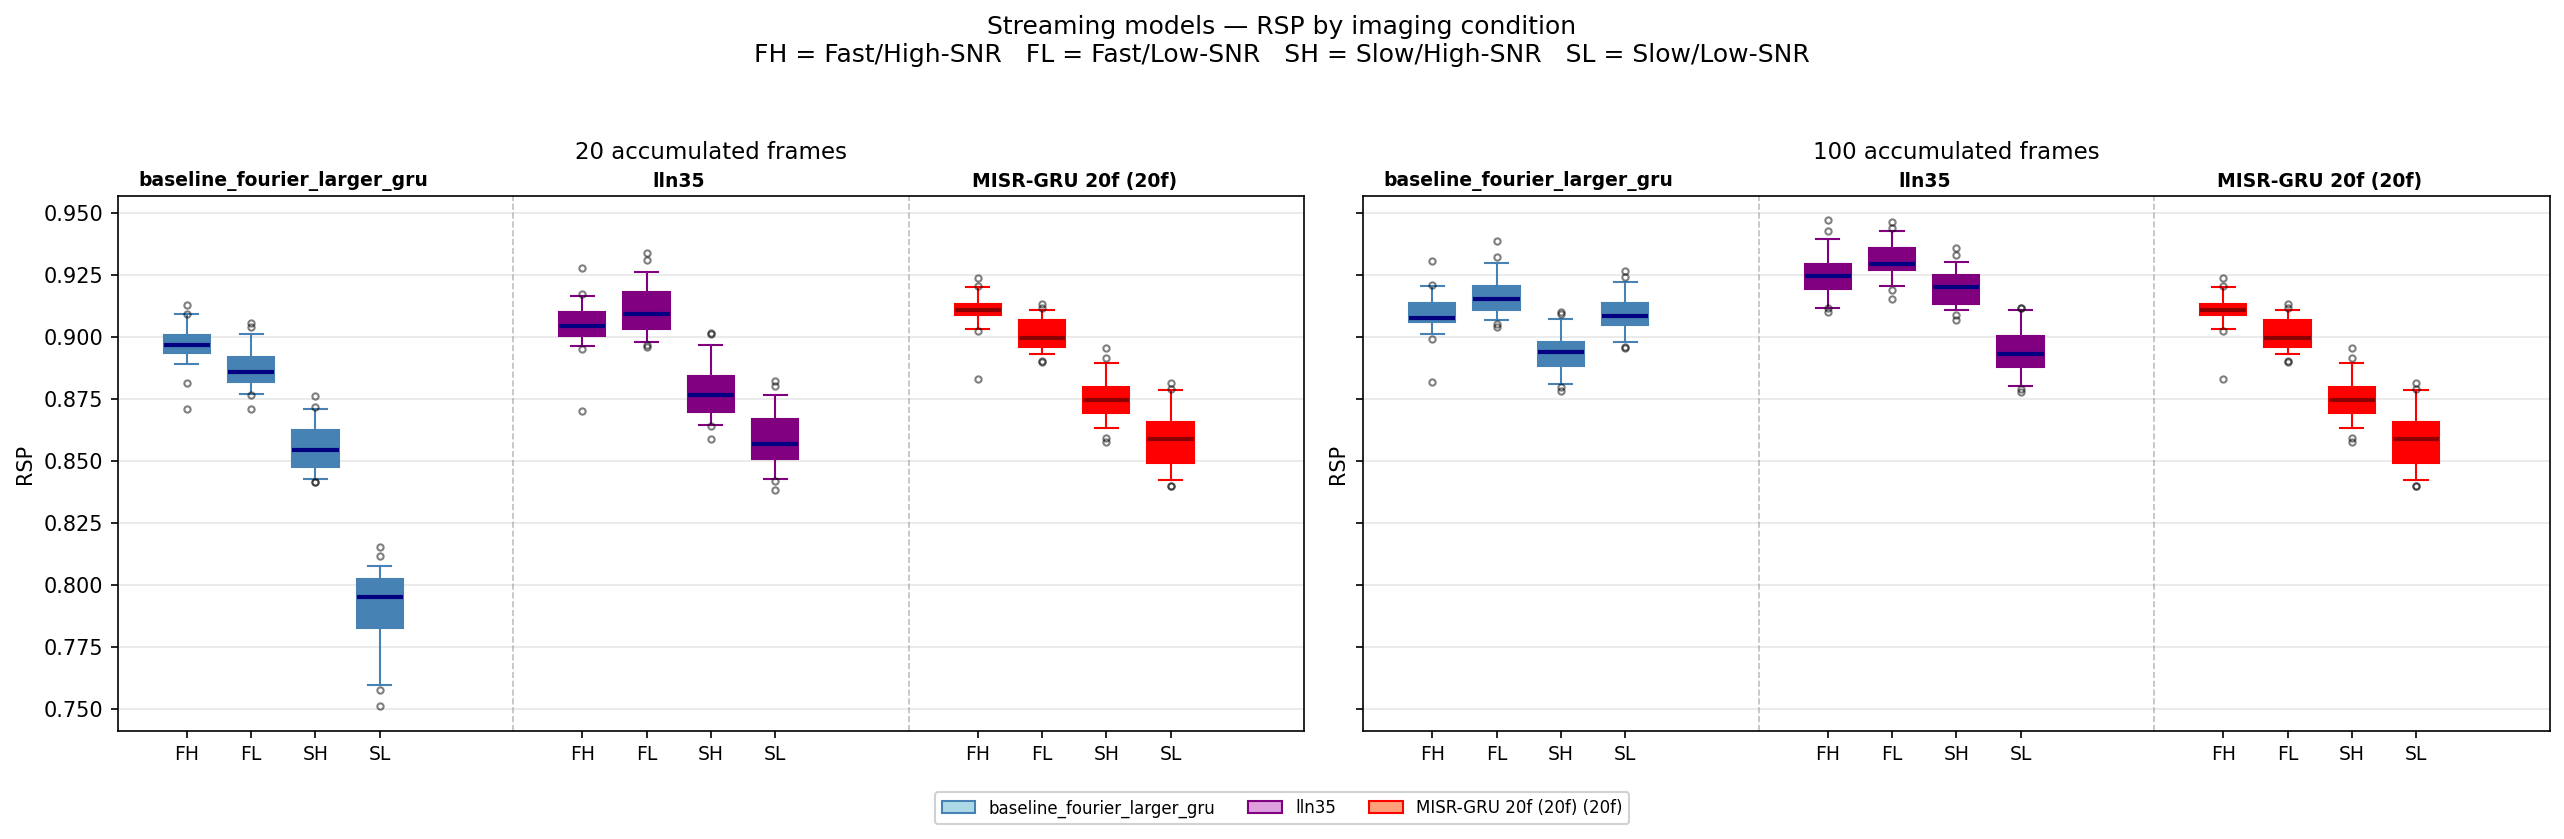
\includegraphics[width=1.0\linewidth]{figures/snr_conditions_streaming_models.png}
  \caption{Performance of two best streaming modelsmodels
and SOFI. Each column corresponds to a different SNR (photons/frame): 100(high-SNR) or 40 (low-SNR), and
and blinking conditions (on time/ off time in ms): 10/600 (fast) or 10/2400 (slow). 
Corresponded resolution estimations and RSP scores of
the models for different conditions. RSP analysis is compared with reference ground-truth (GT),
 a FH: Fast high SNR, FL: Fast low SNR,
SH: Slow high SNR, SL: Slow low SNR}
  \label{fig:lln35_vs_largergrufourier}
\end{figure}
\todo{after greenlight we are planning to retrain one final one using all params
on Miyases account for 48h until fully converge as from the tensorboard logs
the models seem to benefit from more training}

\begin{figure}[h]
  \centering
  \begin{subfigure}[t]{0.48\linewidth}
    \centering
    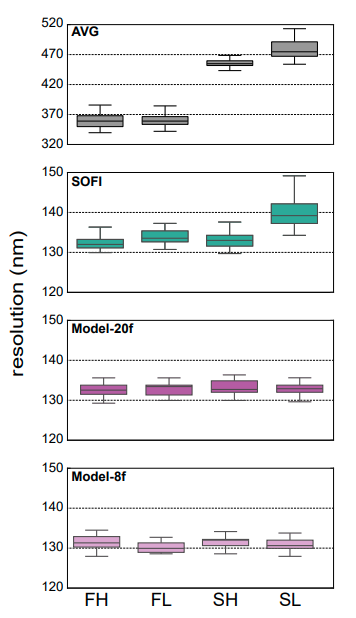
\includegraphics[width=\linewidth]{figures/imdecor_resurf_models.png}
    \caption{Decorrelation analysis of RESURF models (AVG, SOFI, Model-20f, Model-8f).}
    \label{fig:imdecor_resurf}
  \end{subfigure}
  \hfill
  \begin{subfigure}[t]{0.48\linewidth}
    \centering
    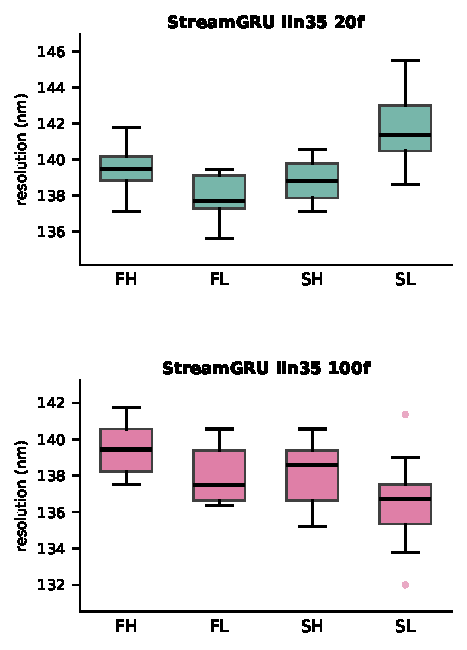
\includegraphics[width=\linewidth]{figures/imdecor_comparison_lln35.pdf}
    \caption{Decorrelation analysis of our trained models across SNR conditions.}
    \label{fig:imdecor_lln35}
  \end{subfigure}
  \caption{Side-by-side decorrelation analysis: RESURF baseline models (left) vs.\ our
           models (right) across FH, FL, SH, and SL blinking/SNR conditions.
           Lower resolution values indicate sharper super-resolved images.}
  \label{fig:imdecor_comparison}
\end{figure}





% \subsection{Practical Implications for Real-Time Imaging}

% These results have direct implications for live-cell imaging deployment. The \texttt{kbuf\_K20} model offers \emph{deterministic} 20-frame-quality reconstruction after exactly 20 acquired frames, with one SR output per subsequent frame at the acquisition frame rate. At 40\,fps, this corresponds to a 0.5\,s warm-up period followed by continuous SR output — sufficient for most live-cell protocols.

% The \texttt{streaming\_fourier} model offers \emph{improving} quality as more frames accumulate, making it better suited to longer recordings or post-acquisition replay. Its slight outperformance of the batch model (Pearson +0.004) suggests that frame-by-frame Fourier supervision acts as an implicit regulariser, encouraging the hidden state to maintain high-frequency information at each step rather than deferring reconstruction quality to the end of the sequence.

% Both streaming models exceed the 8-frame RESURF baseline within 10 accumulated frames, confirming that streaming deployment does not require sacrificing the reconstruction quality established by~\cite{jelle2024}.

\subsection{Streaming Inference Latency}
\label{ssec:streaming_latency}

The architectural distinction between batch and streaming inference has a direct consequence
on throughput: the batch MISRGRU consumes $N$ frames and outputs a single SR
image, whereas the streaming variant emits one SR output for every input frame.
Models were benchmarked on an NVIDIA RTX A5000 using $512\times512$ input frames,
5 warmup passes, and 20 timed passes.

\begin{table}[h]
  \centering
  
  \begin{tabular}{lrccc}
    \hline
    \textbf{Model} & \textbf{Params}
      & \textbf{Total / seq (ms)}
      & \textbf{SR outputs}
      & \textbf{Per SR frame (ms)} \\
    \hline
    Streaming MISRGRU      &  95,073 & $225.90 \pm 0.42$ & 20 & \textbf{11.29} \\
    Streaming Larger GRU   & 131,361 & $240.44 \pm 0.67$ & 20 & 12.02 \\
    Streaming MISRGRU DPA  & 151,996 & $349.26 \pm 0.86$ & 20 & 17.46 \\
    \hline
    Batch MISRGRU (ref.)   &  95,073 & $170.29$          &  1 & 170.29 \\
    \hline
  \end{tabular}
  \caption{Streaming model parameter counts and PyTorch inference latency on $512\times512$
           images (mean over 20 runs, sequence length $N=20$). The \emph{per-frame} column
           divides the total sequence time by the number of SR outputs produced.
           Batch MISRGRU (reproduced from Table~\ref{tab:inference_latency}) is included
           as a reference; it produces only one SR output from 20 input frames.}
  \label{tab:streaming_latency}
\end{table}

All three streaming variants are dramatically more efficient when it comes to producing reconstructed outputs,
while reaching the same accuracy as batched MISRGRU at 20th frame and improving the accuracy with more frames.
The base Streaming MISRGRU takes only 11.32\,ms to produce each SR frame, 
MISRGRU's 170.29\,ms-per-output at the same frame count.
This makes streaming MISRGRU variants very efficient in reconstructing the whole acquisition.

The overal reconstruction of 20 frames is 50ms slower compared to batch MISRGRU but this is due calling
decoding layer 20 times rather than once.

Tje next section~\ref{sec:alignment_ablation} discusses effects of modified MISRGRU with DPA alignment
and finetuning the baseline streaming MISRGRU to reconstruct motion.


% This improvement arises not from a reduction in computation but from amortising the
% processing cost over all 20 outputs: the convolutional GRU processes one frame at a time
% in a fixed-cost forward pass, spreading the total 226\,ms across 20 SR reconstructions
% instead of accumulating 20 frames before a single decode.




\section{Motion reconstruction}
\label{sec:alignment_ablation}
With ultrafast (11ms inference per frame) streaming MISRGRU we decided to explore motion
reconstruction capabilities. 

To evaluate whether explicit inter-frame alignment improves the streaming GRU, we trained
an additional variant incorporating the Deformable Phace-space Alignment module (DPA) inspired by \cite{qiao2025dpatisr}.  

The exact implementation details are described in 

TODO plots
rsp by imaging condition at different speeds (0.2, 1)
compare to static imaging rsp
visual comparison



\paragraph{Real-time deployment feasibility.}
Live-cell fluorescence microscopy typically acquires at 40\,fps (25\,ms budget per frame).
A streaming model must return one SR output within this budget to avoid back-pressure on
the acquisition pipeline.
All three streaming models satisfy this constraint:

\begin{itemize}
  \item \textbf{Streaming MISRGRU} (11.32\,ms) leaves 54\% of the 25\,ms budget unused,
        providing headroom for data transfer, post-processing, or display.
  \item \textbf{Streaming Larger GRU} (12.02\,ms) achieves similar throughput with a
        38\% larger model, confirming that the extra capacity buys marginal reconstruction
        quality without compromising real-time operation.
  \item \textbf{Streaming MISRGRU DPA} (17.46\,ms) includes the deformable alignment
        module (Section~\ref{sec:alignment_ablation}), which adds approximately 6\,ms
        of overhead. The model still meets the 40\,fps budget, but its quality advantage
        over the base model was shown to be negligible (Section~\ref{sec:alignment_ablation}),
        making the extra cost unjustified.
\end{itemize}

Compared to the original SOFI pipeline, which requires on the order of hundreds of frames
and several seconds of off-line processing, the streaming deployment at 11--17\,ms per SR
output represents an acceleration of well over two orders of magnitude, consistent with the
400-fold latency reduction reported for the foundational batch model by~\cite{resurf2024}.
Crucially, the streaming model achieves this at \emph{every frame} rather than at the end
of a fixed acquisition window, enabling truly continuous super-resolution output
synchronised with the microscope acquisition clock.